\documentclass[12pt]{article}
\usepackage{fullpage}
\usepackage{subcaption,amsmath,amssymb,mathtools,xparse,graphicx,float,datetime,color,array,graphics,enumerate,tikz,pgfplots,xcolor}
\usepgfplotslibrary{statistics}
\pagestyle{empty}
\newcommand{\D}{\displaystyle}
\setlength{\textheight}{9in} \setlength{\headheight}{.2in}
\setlength{\headsep}{0in} \setlength{\topmargin}{0in}
\begin{document}
\begin{center}
CSCI 6100 Machine Learning From Data\\
Fall 2018\\
\end{center}
\begin{center}
HOMEWORK 7\\
Daniel Southwick\\
661542908\\
southd@rpi.edu
\end{center}
\vspace{.1in}

\noindent {\bf 1. Classifying Handwritten Digits: 1 vs. 5} \\\\
\indent a) From Problem 3.6(c), we have developed a linear program for nonlinear separable data, which is the same as Problem 3.5. The $optimproblem$ function from Matlab was used to do the following minimization
\begin{center}
$\displaystyle \min_w \sum_{i = 1}^{N}\max (0,1-y_nw^Tx_n)$
\end{center}
The computed result vector is $w_{linear} = \left[ 4.5225 1.0666, -13.3283 \right]$ and we plotted\\$\displaystyle \frac{(w_{linear}(1)+w_{linear}(2)*x)}{w_{linear}(3)}$ with $x$ in the same range as the data intensity range, and resulted the following for the training set and the testing set of data: 
\begin{figure}[H]
  \centering
  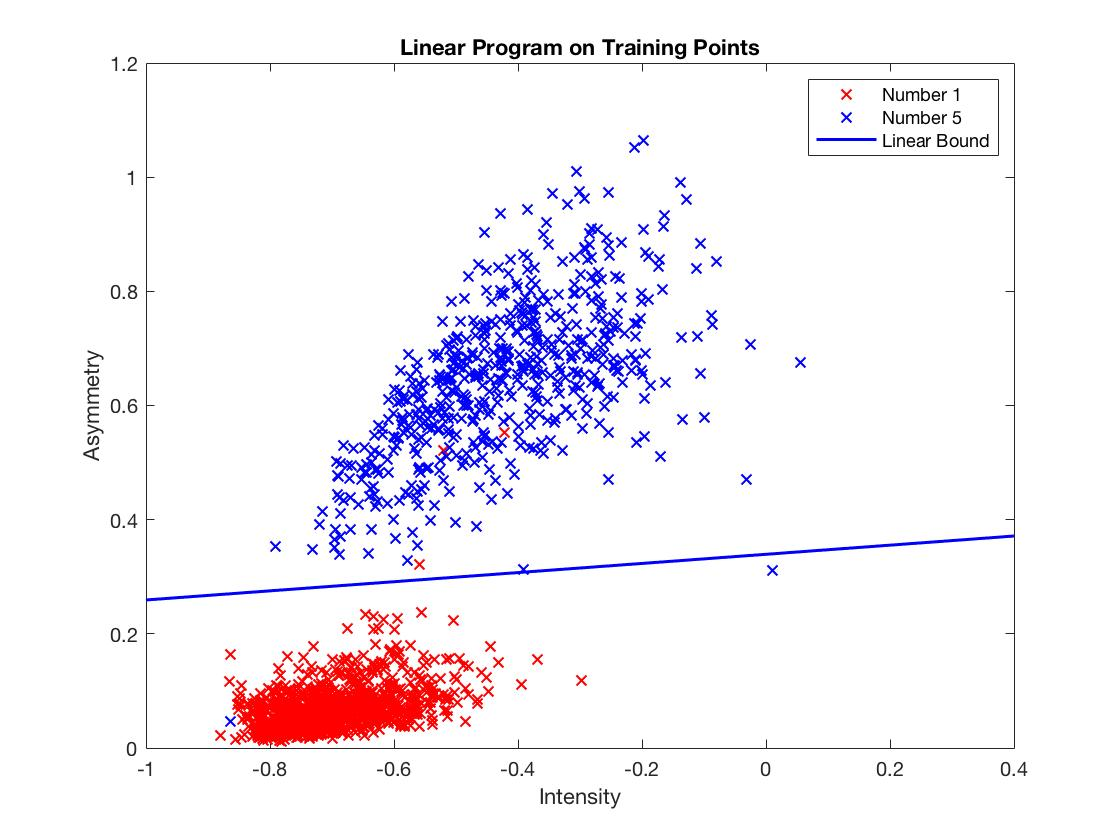
\includegraphics[scale = 0.3]{Pic1.jpg}
  \caption{Linear Program on Training Points}
  \label{fig:Pic1}
\end{figure}
\begin{figure}[H]
  \centering
  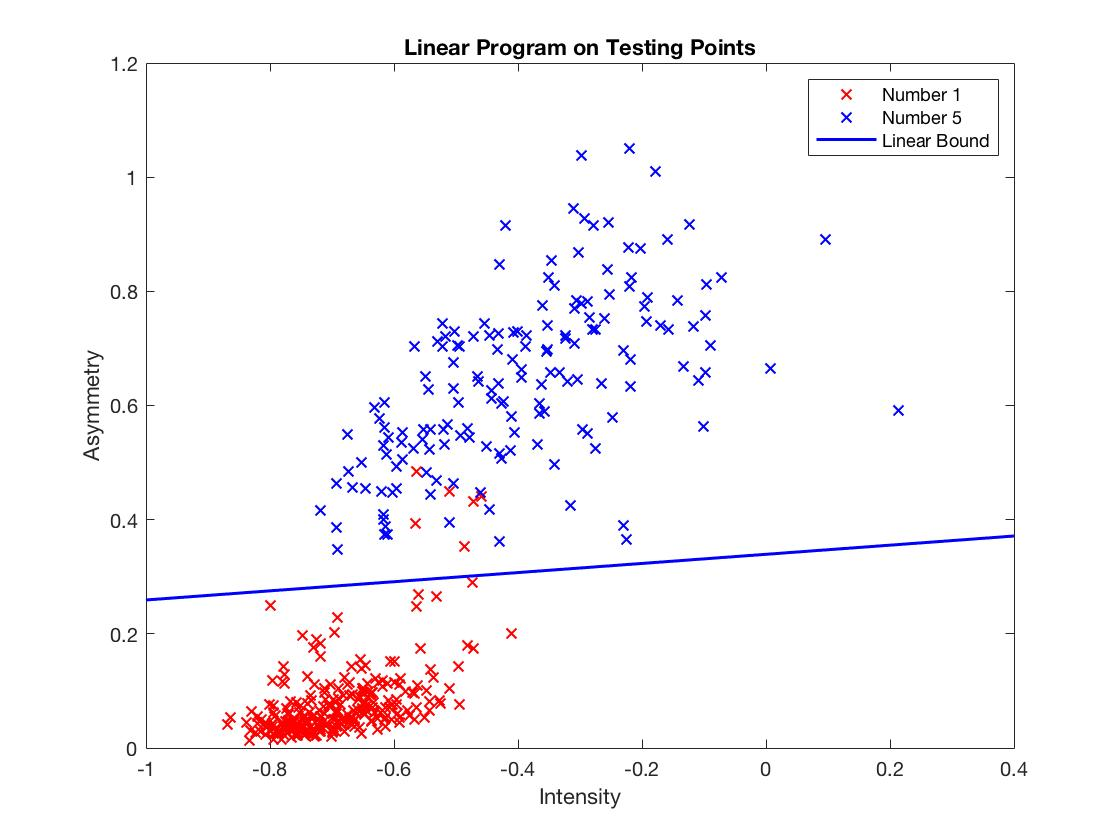
\includegraphics[scale = 0.3]{Pic2.jpg}
  \caption{Linear Program on Testing Points}
  \label{fig:Pic2}
\end{figure}
b) We can compute the error by simply counting the number of misclassified samples and divide by the total sample numbers, since we are only considering $+1$ and $-1$'s to categorize our decision. There are 3 numbers of digit 1 and 2 numbers of digit 5 got misclassified in the training points. so the in sample error:
\begin{center}
$\displaystyle E_{in} = \frac{3+2}{1005+556} = 0.0032$
\end{center}
And there are 6 numbers of digit 1 and 0 numbers of digit 5 got misclassified, so the out sample error:
\begin{center}
$\displaystyle E_{out} = \frac{6+0}{264+160} = 0.0142$
\end{center} \indent\\
\indent c) For the training set, there are total of 1561 points and 2 features so:
\begin{align*}\displaystyle
	N &= 1561, \qquad \delta = 0.05 \\
	d_{vc} &= 2+1 = 3 \\
	E_{out} & \leq E_{in} + \sqrt{ \frac{8}{N}\ln\left(\frac{4( (2N)^{d_{vc}}+1 )}{\delta}\right) } \\
	& \leq E_{in} + \sqrt{ \frac{8}{1561}\ln\left(\frac{4( 3121^3+1 )}{0.05}\right) } \\
	& = 0.0032 + 0.382310 \\
        E_{out} &  = 0.385510
\end{align*}
For the testing set, there are total of 424 points:
\begin{align*}\displaystyle
	N &= 424, \qquad \delta = 0.05 \\
	d_{vc} &= 2+1 = 3 \\
	E_{out} & \leq E_{in}+\sqrt{\frac{1}{2N}\ln \frac{2M}{\delta}}\\
	& \leq E_{in}+\sqrt{\frac{1}{848}\ln \frac{2}{0.05}}\\ 
	& = 0.0142 + 0.065955 \\
	E_{out} & =  0.080155
\end{align*}
The bound on the testing set is much better than the bound on the training set.\\\\
\indent d) We apply the 3rd order polynomial transform to the existing method by implementing $\Phi(x)=(1,x_1,x_2,x_1^2,x_2^2,x_1x_2,x_1^3,x_2^3,x_1x_2^2,x_1^2x_2)$ and resulted the following for the training set and the testing set of data: 
\begin{figure}[H]
  \centering
  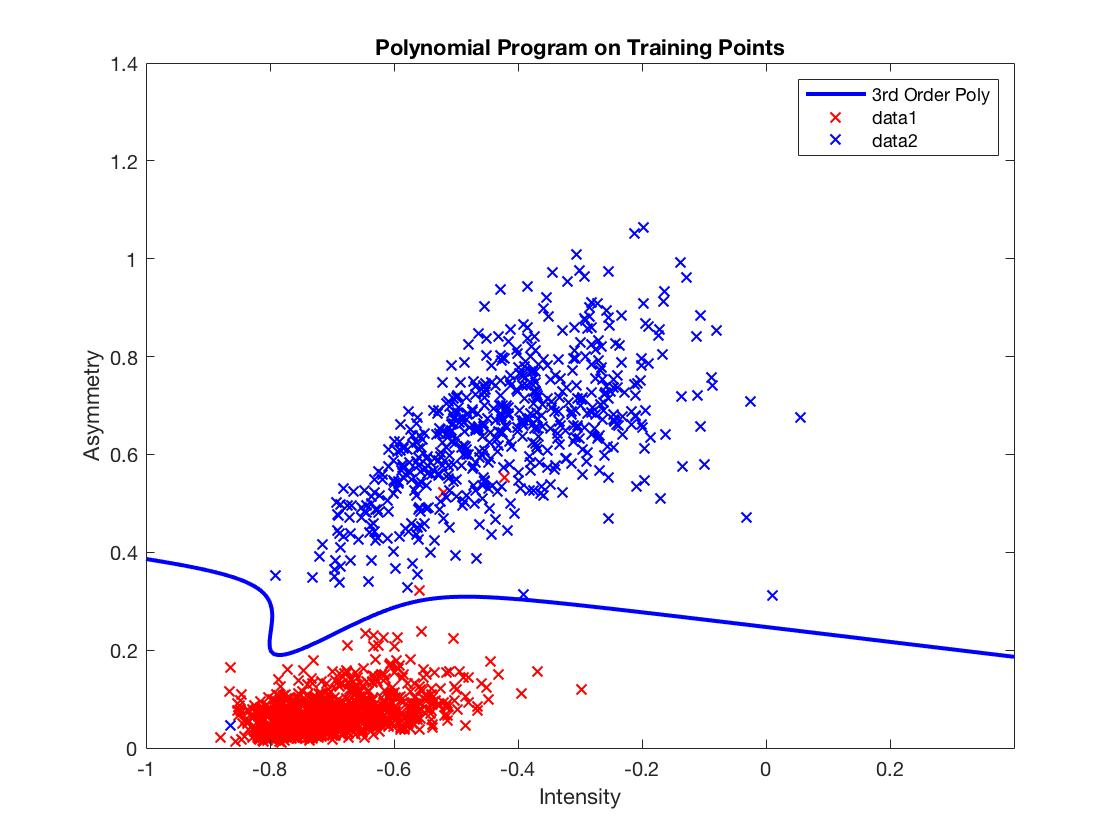
\includegraphics[scale = 0.3]{Pic3.jpg}
  \caption{Quadratic Program on Training Points}
  \label{fig:Pic3}
\end{figure}
\begin{figure}[H]
  \centering
  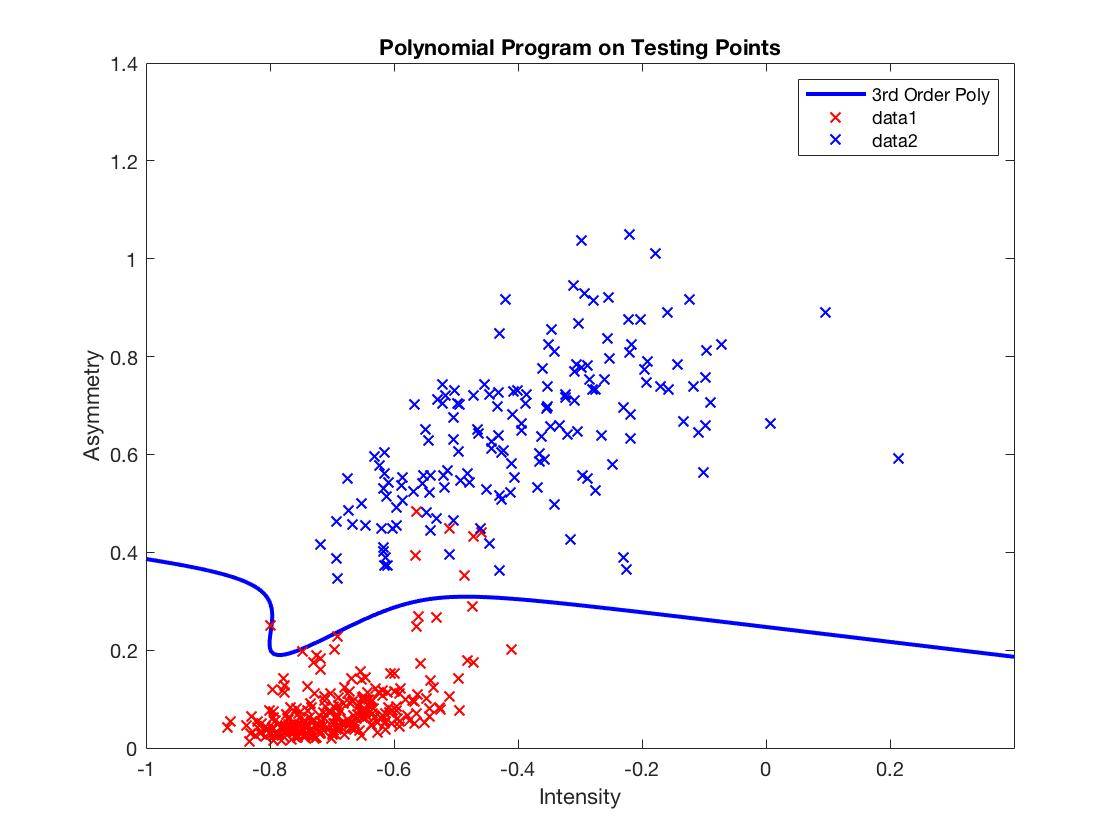
\includegraphics[scale = 0.3]{Pic4.jpg}
  \caption{Quadratic Program on Testing Points}
  \label{fig:Pic4}
\end{figure}
Then, there are 3 numbers of digit 1 and 1 numbers of digit 5 got misclassified in the training points. so the in sample error:
\begin{center}
$\displaystyle E_{in} = \frac{3+1}{1005+556} = 0.0026$
\end{center}
And there are 6 numbers of digit 1 and 0 numbers of digit 5 got misclassified, so the out sample error:
\begin{center}
$\displaystyle E_{out} = \frac{6+0}{264+160} = 0.0142$
\end{center}
and for the training, testing $E_{out}$ with a new $d_{vc} = 10$
\begin{align*}\displaystyle
	N &= 1561, \qquad \delta = 0.05 \\
	d_{vc} &= 2+1 = 3 \\
	E_{out} & \leq E_{in} + \sqrt{ \frac{8}{N}\ln\left(\frac{4( (2N)^{d_{vc}}+1 )}{\delta}\right) } \\
	& \leq E_{in} + \sqrt{ \frac{8}{1561}\ln\left(\frac{4( 3121^{10}+1 )}{0.05}\right) } \\
        E_{out} &  = 0.662032
\end{align*}
\begin{align*}\displaystyle
	N &= 424, \qquad \delta = 0.05 \\
	d_{vc} &= 2+1 = 3 \\
	E_{out} & \leq E_{in}+\sqrt{\frac{1}{2N}\ln \frac{2M}{\delta}}\\
	& \leq E_{in}+\sqrt{\frac{1}{848}\ln \frac{2}{0.05}}\\ 
	& = 0.0142 + 0.065955 \\
	E_{out} & =  0.080155
\end{align*}
e) So I would definitely prefer using the linear model, since the 3rd order polynomial transform did not only result in worse performance on testing set, but also gives a higher bound of $E_{out}$ theoretically, due to the increasing of $VC$ dimension. So in this case, a simpler model is better. \\\\\\\\

\noindent {\bf 2. Gradient Descent on a "Simple" Function} \\\\
\begin{align*}\displaystyle
f(x,y)&=x^2+2y^2+2\sin(2\pi x)\sin(2\pi y)\\\\\\
\nabla f(x,y)&=
\begin{bmatrix}
2x+4\pi \cos(2\pi x)\sin(2\pi y)\\
4y+4\pi \sin(2\pi x)\cos(2\pi y)
\end{bmatrix}\\\\\\
\begin{bmatrix}
x_{t+1}\\
y_{t+1}
\end{bmatrix}
&=
\begin{bmatrix}
x_{t}\\
y_{t}
\end{bmatrix}
-\eta
\begin{bmatrix}
2x_t+4\pi \cos(2\pi x_t)\sin(2\pi y_t)\\
4y_t+4\pi \sin(2\pi x_t)\cos(2\pi y_t)
\end{bmatrix}
\end{align*}\\\\\\
\indent a) We applied the above gradient descent algorithm with $\eta = 0.01$ and $\eta = 0.1$ and obtained the following results:
\begin{figure}[H]
  \centering
  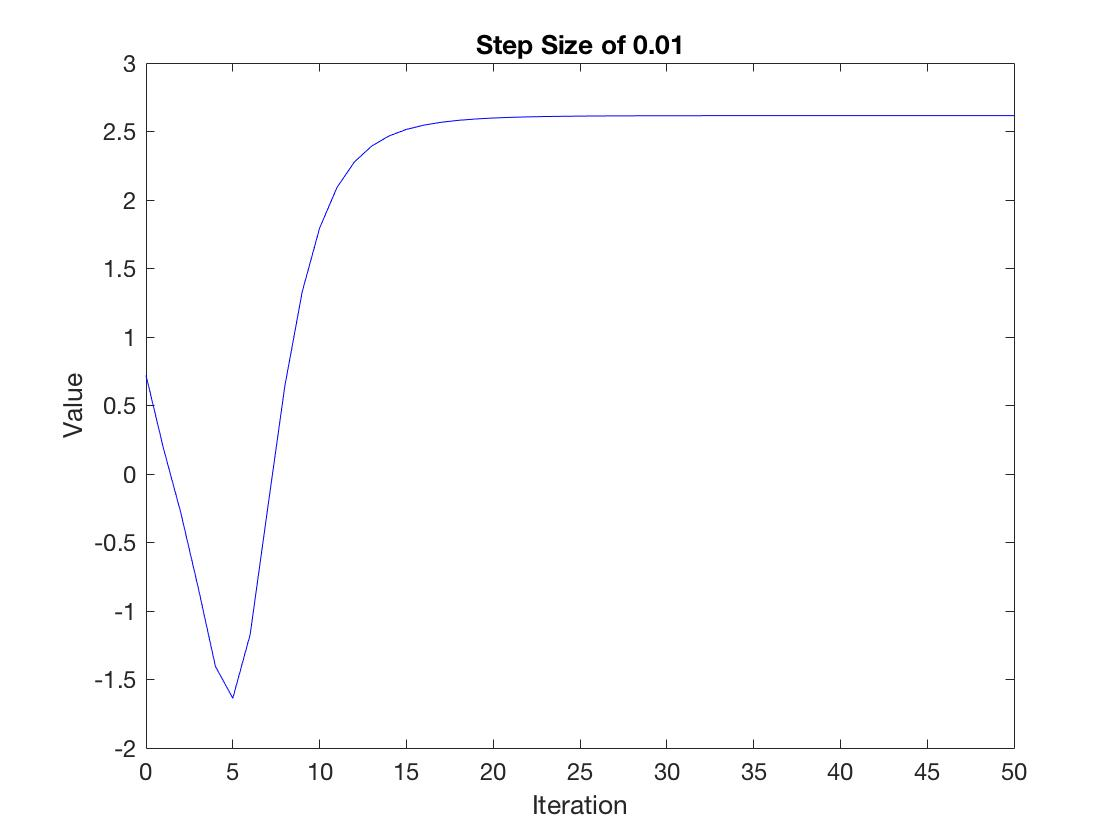
\includegraphics[scale = 0.3]{Pic5.jpg}
  \caption{Gradient Descent with $\eta = 0.01$}
  \label{fig:Pic5}
\end{figure}
\begin{figure}[H]
  \centering
  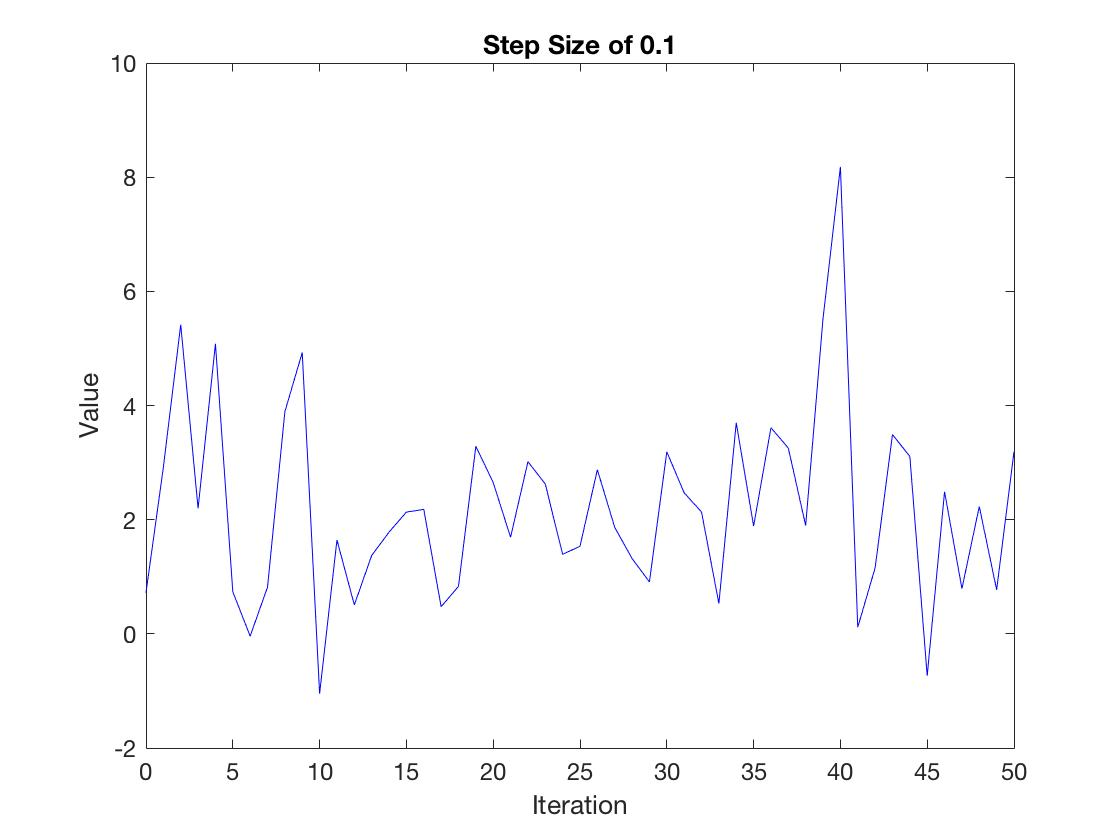
\includegraphics[scale = 0.3]{Pic6.jpg}
  \caption{Gradient Descent with $\eta = 0.1$}
  \label{fig:Pic6}
\end{figure}
\begin{table}[H]
 	\label{Table: minimum values}
 	\centering
 	\begin{tabular}{c|c|c|c|c}
 		\hline
 		\text{Initial points} & \multicolumn{2}{c}{$\eta=0.01$} & \multicolumn{2}{c}{$\eta=0.10$}\\
 		\cline{2-5}
 		$(x_0,y_0)$ & $f(x^*,y^*)$ & $(x^*,y^*)$ & $f(x^*,y^*)$ & $(x^*,y^*)$ \\
 		\hline
 		(0.1,\ 0.1) & -1.6365 & (-0.2807,\ 0.1809) & -1.0492 & (-0.6476,\ -0.2554) \\
 		\hline
 		(1,\ 1) & 2.5926 & (0.9800,\ 0.8437) & -1.7419 & (-0.2475,\ 0.2812)  \\
 		\hline
 		(-0.5,\ -0.5) & 0.7500 & (-0.5,\ -0.5) & -1.3272 & (0.7367,\ 0.2479)  \\
 		\hline
 		(-1,\ -1) & 2.5926 & (-0.9800,\ -0.8437) & -1.7419 & (0.2475,\ -0.2812) \\
 		\hline
 	\end{tabular}\vspace{-3mm}
\end{table}\indent \\
\\We can see that the function converged with $\eta = 0.01$ and bounced around when $\eta = 0.1$, This is mainly caused by the step size. A smaller step size leads to a higher computation cost, but if the step size is not small enough, the function value will be trapped in the local minimum region thus not leading to the global minimum.\\\\

\noindent {\bf Problem 3.16} \\\\
\indent a) Since $\mathbb{P}[y = +1 \big| \textbf{x}] =g(\textbf{x})$, thus $\mathbb{P}[y = -1 \big| \textbf{x}] = 1-g(\textbf{x})$. So:
\begin{align*}
	\mbox{Predicted}(+1) & \mbox{ and actual }y = -1:\\
	\mbox{cost(accept)} &= (1-g(\textbf{x}))c_a\\
	\mbox{Predicted}(-1)&  \mbox{ and actual }y = +1:\\
	\mbox{cost(reject)} &= g(\textbf{x})c_r
\end{align*}
\indent b)So if the cost of reject $\geq$ the cost of accept, we choose to accept the person:
\begin{align*}\displaystyle
		g(\textbf{x})c_r &\geq (1-g(\textbf{x}))c_a \\
		g(\textbf{x})(c_r+c_a) &\geq c_a \\
		g(\textbf{x}) &\geq \frac{c_a}{c_r+c_a} \\
		\kappa &= \frac{c_a}{c_r+c_a} \\
		\mbox{And } g(\textbf{x}) &\geq \kappa\\
		\mbox{Thus } \kappa &= \frac{c_a}{c_r+c_a}
\end{align*}
\indent c)
	\begin{center} \begin{tabular}{cc  cccc cc}
	&Supermarket&&&&CIA\\
		&\begin{tabular}{c |  c c}
			&$+1$&$-1$\\\hline
			$+1$&$0$&$1$\\
			$-1$&$10$&$0$
		\end{tabular} 
		&&&&\begin{tabular}{c | c c}
			&$+1$&$-1$\\\hline
			$+1$&$0$&$1000$\\
			$-1$&$1$&$0$
		\end{tabular} \\\\
		&$\displaystyle\kappa = \frac{1}{1+10} \approx  0.0909$
		&&&&
		$\displaystyle\kappa = \frac{1000}{1+1000} \approx 0.9990$\\\\
	\end{tabular} \end{center}
\indent The threshold value $\kappa$ should be higher if the target focus more on the safety level, in this case, it's ok for supermarket to accept some false targets, but for CIA, intruders can cause serious problems.
\end{document}

